\documentclass[a4paper,12pt, oneside, openright, draft]{report}
\hyphenpenalty=5000
\usepackage{graphicx}
\usepackage{float}
\usepackage{url}
\usepackage{indentfirst}
\usepackage{nomencl}
\usepackage{fixme}

\makenomenclature
\floatstyle{boxed} 
\restylefloat{figure}

\begin{document}
%-----------------
\begin{titlepage}
\newcommand{\HRule}{\rule{\linewidth}{0.5mm}}
\begin{center}

% Title

{ \huge \bfseries Networking for Smart Meters}\\[0.4cm]
{\large Chaitanya Dandugula}\\
{\small dandu@kth.se}

\vfill

\emph{Examiner:} Professor Gerald \textsc{Q. Maguire Jr.}\\
{Royal Institute of Technology}\\
{Sweden}\\[0.8cm]

\emph{Supervisor:} Peter \textsc{Schoo}\\
{Fraunhofer Research Institution for Applied and Integrated Security}\\
{Germany}\\[0.8cm]

% Bottom of the page
{\small \today}

\end{center}

\end{titlepage}
%---------------------

\begin{abstract}

\indent This literature study report is part of the Master's thesis project - ``Networking for Smart Meters''. The report starts by giving a broad overview of the problem that is to be solved and then moves on to different technologies, specifically PLC, 6LoWPAN, and HIP, that can be used to develop the network architecture. Methods for securing the network include the Resurrecting Duckling Policy and the BSI Protection Profile. These methods are discussed before concluding the report with a summary of the previous work done in this field. 

The result of this literature study will be the base for further work and implementation of a proof-of-concept based on the chosen network architecture. 

\end{abstract}
%Table of Contents

\tableofcontents
\listoffigures
\listoftables
\renewcommand{\nomname}{List of Abbreviations}
\printnomenclature[2.5cm]
\nomenclature{SMS}{Smart Metering System}
\nomenclature{SM}{Smart Meter}
\nomenclature{PLC}{Power Line Communication}

%Chapter 1: Introduction
\chapter{Introduction}
\section{Overview}
A Smart Metering System (SMS) is composed of many Smart Meters (SM), devices that measure the consumption or production of commodities like electrical energy, gas, or water in a physical metrological measurement metering unit and transform the measured values into digital information, that can eventually be forwarded to an accounting system, and further to a billing system. A data collector  called a Gateway is used for the collection of the metered data from the SMs and  forward the data to the accounting systems operated by one enterprise, which then delivers the accounting information to another enterprise. For example, a power distribution operator  might collect the accounting information and provide it in aggregated form to the power supply company. Since recently\footnote{March, 2011} there is a Protection Profile (PP) for the Gateway proposed by the German Federal Office for Information Security (BSI) \cite{BSI_pp} that sets out the security requirement for the SM networks in Germany and in this process defines a reference network architecture.

The communication between the SMs and the Gateway is unmanaged, requiring self-configuration support, confidentiality of the communicated information, and may need to take place in a hostile environment. Whereas the communication between the Gateways and the accounting system is managed, requires integrity and confidentiality of the communicated accumulated information, and access to the accounting system by the power generation companies is regulated.

The idea is now to utilize HIP \cite{HIP_rfc} to initiate IPsec protected communication, such that asymmetric keys, generated on smart meters, are used as identifier and that the Gateway accepts the meter as its slave, according to the Resurrecting Duckling security policy \cite{Sta_duck}. It is assumed that the Gateway can be identified to the accounting system by asymmetric keying material managed by means of a Public Key Interface (PKI).

\section{Problem statement}
The aim of this thesis project is to  enhance network security domains so that communication in future smart metering provides secure auto-configurable HIP-enable networks with  a self-generated cryptographic identifier so that a SM can communicate via a Gateway.

The thesis project can be divided into the following three phases:
\begin{itemize}
\item Literature study: to study the different network architectures, communication protocols and technologies suitable for smart meters. 
\item Designing: this phase encompasses the overall design of a demo network scenario suitable for implementation.
\item Implementation: to implement the proof-of-concept in a lab environment and to validate/test the same against security threats and performance.
\end{itemize}

%Chapter 2: Technological Alternatives
\chapter{Technological Alternatives}
\section{Power Line Communication (PLC)}

Power Line Communication (PLC) is a technology for data communication on a conductor used also for carrying electric power. PLC systems operate by impressing a modulated carrier signal on the power wiring system. The frequency bands used by the PLC systems depends on the power wiring used and the signal transmission characteristics. The metered data can be collected at the consumer's premises and this data can be transmitted over the power lines to the supplier. However since power lines were set up not for the purpose of transmission of data but for the transmission of power, the power wire circuits have limited ability to carry higher frequency signals.

PLC systems provides variable data rates depending on the frequency of the carrier signals used. Single carrier Narrow-Band (NB) provides data rates of few kbps with carrier wave frequency varying from 20 to 200 kHz. On the other hand, Broad-Band systems (BB), operating at higher frequencies (2-30 MHz),  provide data rates of upto 200 Mbps \cite{PLC_galli}. NB-PLC and BB-PLC provide a platform for bi-directional communication and are capable of handling real-time data thus enabling utilities to identify and even predict equipment failures. There is considerable evidence that PLCs can provide point-to-point configurations on the Medium Voltage (MV) segment of the distribution grid and point-to-multipoint configurations on the Low Voltage (LV) segment of the distribution grid \cite{PLC_galli}.

Although PLC based Advanced Metering Infrastructure (AMI) has a proven track record, it lacks  standardization and this could be a major factor with respect to the large scale commercial adaptation of PLC systems for AMI \cite{PLC_galli}. The power line channel is frequency selective, time-varying and noisy, this implies the channel is difficult to model. There is also the problem of jumping too quickly onto the bandwagon of Smart Grid (SG) applications with the wrong PLC technology.

Apart from the technical aspects of PLC systems, there are various governmental regulations and business requirements that dictate the mass acceptance of the technology. For example, the EU regulations does not allow for the use of BB-PLC due to stricter limitations on the allowable transmit power. The significant advantage of PLC systems is that the common conception of separated functions of sensing and communication blend together and thus does not require the installation of another communication channel. Due to the existing infrastructure for the distribution of power through power line, it is not hard to imagine that PLC systems have a deployment costs comparable to wireless technologies. 

\subsection{IPv6 and PLC}

IPv6 with PLC, an idea using the IEEE 802.15.4 standard \cite{IEEE_802.15} for the physical layers and building an IPv6 stack on top of it. Although the IEEE 802.15.4 standard is for the wireless medium at the physical layer, successful adaptation of the standard to the power line medium at the physical layer are presented in \cite{IP_PLC}. IPv6 extends the IP address space from 32 to 128 bits and solves some very important issues, like auto configuration, security and multicasting. This is increasingly necessary in the growing “Internet of things”.

The proof-of-concept implementation of IPv6 over PLC \cite{IP_PLC}, uses PLC nodes that are architecturally similar to the classic RF 802.15.4 nodes. These nodes are powered by micro-controllers and the communication is handled by a PLC transceiver which emulates a radio transceiver. The micro-controller deals with the compliance of 802.15.4 data format and the upper layers of the communication stack while the transceiver provides a throughput of 10 kbps that induces some adaptation within the MAC part. These adjustments provide a communication on power line with 802.15.4 frame format. Furthermore, an IPv6 stack has a memory foot print of approximately 13 kB, and an OS that provides a complete IPv6 network stack has a foot print of 40 kB \cite{IP_PLC}.

\section{IPv6 over Low power Wireless Personal Area Networks (6LoWPAN)}

Low-power and Lossy Networks (LLNs) refer to networks that are composed of highly constrained nodes (limited power, memory and CPU) connected by ``lossy" links (low power radio links or PLC). A LoWPAN is a particular type of LLN, formed by devices/nodes complying with the IEEE 802.15.4 standard. The 6LoWPAN standard provides for head compression and encapsulation mechanism, that allow IPv6 packets to be sent to and received from, over IEEE 802.15.4 based networks.

Typical characterisitcs of LoWPAN nodes \cite{6LPN_dna_draft,6LPN_prob_rfc}:
\begin{itemize}
\item Short range: The operating range of the nodes is about 10 meters.
\item Low power: The transmission power of the nodes is set at around 0 to 3dBm.
\item Low memory: The nodes have typically around 512 KB of Flash memory.
\item Limited processing power: Although certain models exist with 16-bit and 32-bit cores, the smallest common nodes have 8-bit processors with clock rates around 10 MHz.
\item Low bit rate: A maximum over-the-air data rate of 250 kbps is achieved by most of the nodes.
\end{itemize}

Furthermore, the idea of IP over PLC could be strengthened by using 6LoWPAN for header compression and the Routing Protocol for Low power and Lossy Networks (RPL\footnote{http://tools.ietf.org/wg/roll/draft-ietf-roll-rpl}) as  a routing protocol. RPL is not limited to any particular link layer and can be used for low power wireless or PLC. However, RPL is still in draft stage and provides no security features, hence this could be a shortcoming.

\subsubsection{6LoWPAN over ZigBee}
ZigBee\footnote{ZigBee Alliance - http://www.zigbee.org} has access to two large markets and has standards in place for device interoperability, on the other hand 6LoWPAN has some technical weakness and the standard is still in the draft phase. However, the main advantage of 6LoWPAN over ZigBee is that 6LoWPAN operates on TCP/IP and TCP/IP is the lingua franca of communications all over the world and hence there is no adoption curve associated with 6LoWPAN as it is with ZigBee. This is important as any technology is not only driven by its technical prowess but also by the adoption by the masses. Hence the idea of combining the 6LoWPAN and Zigbee could be a first step in truly creating the ``Internet of things". 

\section {Host Identity Protocol (HIP)}

IP address and DNS names constitute the two important global namespaces. Semantic overloading and functionality extensions have complicated these namespaces and as a result introduced a number of weaknesses. There are three critical deficiencies with the current namespaces.  First, anonymity is not provided in a consistent, trust-able manner. Second, dynamic readdressing cannot be directly managed and finally, authentication for systems and datagrams is not provided.

\begin{figure}[htb!]
\centering
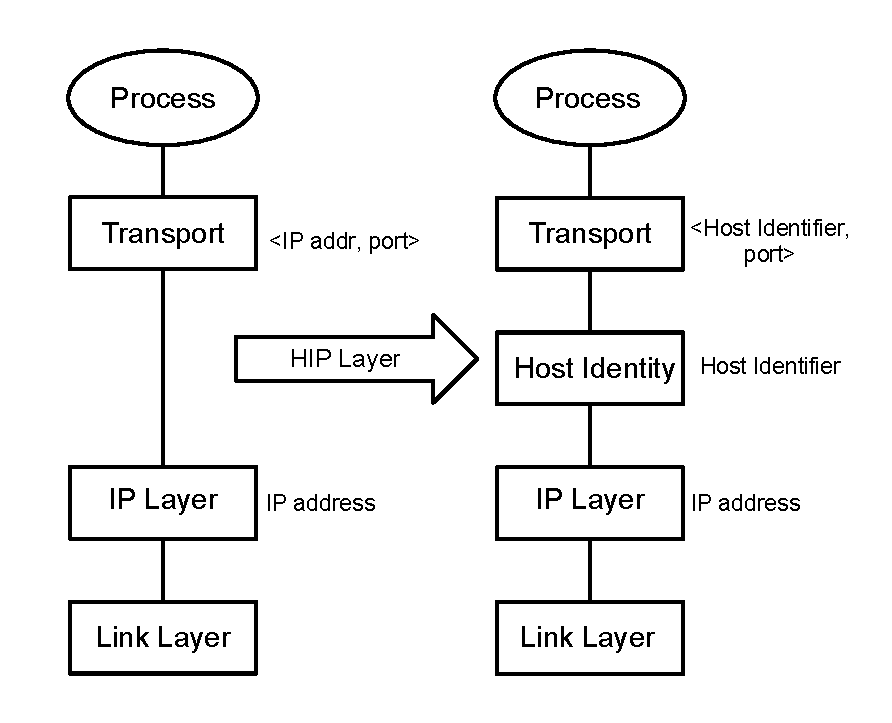
\includegraphics[width=0.8\textwidth]{images/HIP_figure1}
\caption{HIP architecture}
\label{fig:HIP_arch}
\end{figure}

HIP \cite{HIP_rfc} proposes a new namespace consisting of Host Identities and Host Identifiers (HI). There is a subtle but important difference between the two. Host Identifier is cryptographic in nature; it is the public key of an asymmetric key-pair where as a Host Identity refers to an abstract concept assigned to a `computing platform'. Each host is uniquely identified by a Host Identity and a corresponding Host Identifier (see Figure~\ref{fig:HIP_arch}). Note that however a single host can have more than one Host Identity.

In the current IP architecutre, IP addresses act as both locators and end point identifiers. That is, the IP addresses act as a routing direction vector that identifies  topological location in the Internet besides naming the physical network interface at the point-of-attachment. With HIP, the end-point names and locaters are two distinct entities. IP addresses continue to act as locators, while the Host Identifiers correspond to end-point names as shown in Figure~\ref{fig:HIP_arch}. 

With the use of HIP, transport layer protocols are no longer bound to a single IP address but to Host Identities. This enables HIP to provide for process migration and clustered servers.

The main objectives of HIP are to enhance mobility, provide for limited forms of trust between systems, dynamic IP renumbering and multi-homing. The Host Identifiers can be used in many authentication systems, such as the Internet Key Exchange (IKEv2) protocol, thus the payload traffic between HIP host is typically, but not necessarily protected with IPsec and in turn makes these payload IP packets no different from the standard IPsec protected IP packets. In other words, HIP can be seen as a special case of using IPsec thus building on top of the existing IPsec infrastructure.

\subsection{Host Identity Namespace}

A Host Identifier is a name in the Host Identity namespace, Host Identifiers represents a statistically globally unique name for naming any system with an IP stack. Although, any name that claims to be ‘statistically globally unique’ may serve as a Host Identifier, a public key of a public key pair is best recommended for an Host Identifier \cite{HIP_rfc}. 

HIP provides optional cryptographic features, however the protocol with its cryptographic features provides the complete set of functionality as advertised by the RFC. Hence using the public key as the Host Identifier avoids the need for an additional name. The Host Identifiers can be public or private i.e., they can be published or unpublished. The public Host Identifiers are stored in DNS or LDAP directories. Alternatively these identifiers can also be stored in various kinds of Public Key Infrastructure (PKI) and hence extending the scope of a Host Identifier beyond the purpose of host identification.

\subsection{The Protocol Overview}
Normal operation of HIP uses a Host Identity Tag. A HIT is a 128 bit representation of a Host Identity and is a cryptographic hash of the corresponding Host Identifier. The purpose of HIT is to enable a consistent representation of the Host Identity irrespective of the cryptographic algorithms used and to provide easier protocol encoding because of its fixed length. As HIT is used to identify the sender and recipient of a packet, it should be unique in the whole IP universe and in the case of a collision the Host Identifiers (public keys) will make the final difference.

\begin{figure}[htb!]
\centering
\includegraphics[width=0.8\textwidth]{images/HIP_figure2}
\caption{HIP base exchange}
\label{fig:HIP_be}
\end{figure}

The actual Host Identity Protocol (HIP) is composed of two two-round-trip, end-to-end Diffie-Hellman key exchange protocol, a mobility exchange and some additional messages. The purpose of the HIP base exchange (see Figure~\ref{fig:HIP_be}) is to create assurance that the peers indeed possess private keys corresponding to their host identifiers (public keys). In consequence, the base exchange creates a pair of IPsec Encapsulated Security Payload (ESP) Security Associations (SAs), one in each direction.

\begin{figure}[htb!]
\centering
\includegraphics[width=0.8\textwidth]{images/HIP_figure3}
\caption{HIP with DNS}
\label{fig:HIP_DNS}
\end{figure}

Figure~\ref{fig:HIP_be} shows the process of base exchange. First the initiator looks up Host Identifier/HIT of the responder from DNS or RVS (Rendezvous Server). Figure~\ref{fig:HIP_DNS} depicts the procedure for HIP with DNS. On the client side, the application sends DNS query to a DNS server. The DNS server replies with the Host Identifier (FQDN-\textgreater HI) instead of IP address. In a second step, another lookup is made in the Host Identity layer by the HIP daemon. This time, Host Identities are translated into IP addresses (HI-\textgreater IP) for network layer delivery.

The transport protocol sends a packet containing server's Host Identifier. The Host Identity layer replaces the Host Identifier with corresponding IP address of the server. The network layer transmits this packet with an IP header. Accordingly, the 5-tuple socket becomes \{protocol, source HI, source port, destination HI, destination port\} from the conventional \{protocol, source IP, source port, destination IP, destination port\}. 

HIP uses a special IPsec ESP mode called Bound End-to-end Tunnel (BEET). The new mode provides limited tunnel mode semantics without the regular tunnel mode overhead.

\subsection{Mobility}
\begin{figure}[htb!]
\centering
\includegraphics[width=0.8\textwidth]{images/HIP_figure4}
\caption{Mobility with HIP}
\label{fig:HIP_mob}
\end{figure}

Since the SAs are not bound to IP addresses, the host is able to receive packets that are protected using a HIP-created ESP SA from any address. Thus, a host can change its IP address and continue to send packets to its peers. Figure~\ref{fig:HIP_mob} depicts the mobility process. In the beginning, the mobile host is at address 1 and it moves to the address 2 later. During the mobility process, the mobile host is disconnected from the peer host for a brief period of time while it switches from address 1 to address 2. Upon obtaining a new IP address, the mobile host sends a \texttt{LOCATOR} parameter to the peer host in an \texttt{UPDATE} message. The \texttt{LOCATOR} indicates the new IP address, the IPsec - Security Parameters Index (SPI) associated with new IP address, the address lifetime and whether the new address is a preferred address. The peer host performs an address check and solicit a response from the mobile host. Depending on whether the mobile host has initiated a rekey, and on whether the peer host itself wants to rekey to verify the mobile host's new address, the process can be categorized into three cases: 
\begin{itemize}
\item Readdress without rekeying, but with an address check, as in Figure~\ref{fig:HIP_mob}; 
\item Readdress with a mobile-initiated rekey; and 
\item Readdress with a peer-initiated rekey.
\end{itemize}

\subsection{Multihoming}
\begin{figure}[htb!]
\centering
\includegraphics[width=0.8\textwidth]{images/HIP_figure5}
\caption{Multihoming with HIP}
\label{fig:HIP_mhom}
\end{figure}
A host can sometimes have more than one interface. The host may notify the peer host of the additional interfaces by using the \texttt{LOCATOR} parameter. In Figure~\ref{fig:HIP_mhom} the multihoming host is assumed to have two IP addresses, \textit{addr1} and \textit{addr2}. Further, \textit{addr1} is assumed to be the preferred address. The multihoming host sends an \texttt{UPDATE} packet including \textit{addr1} and \textit{addr2} to its peer host. The peer host sends \texttt{UPDATE} packets to each address and updates corresponding SPIs.

%Chapter 3: Security
\chapter{Security}

Security threats can be broadly classified into three main classes, depending on whether the system property being threatened is confidentiality, integrity or availability. The protection schemes to counter these security threats involve a three step process: identification (the user says who she is), authentication (the system verifies the validity of this claim), and authorization (she is granted specific access rights).

\section {Data privacy}

Privacy protection of the metering data from individual SMs is very important for future smart grid and smart metering networks for their roll out and eventual acceptance by the public: research in this area is ongoing and SM users will need to be reassured that their data is secure. The metering data should be securely anonymized and also be securely attributable to a specific location (e.g. a group of houses or  apartments) for billing purposes. The accounting company should not be aware of the association between the individual SM data and the consumer and thus anonymization helps to achieve this task.

The main question regarding the protection of privacy of individual customers becomes: How can high-frequency data be anonymized, i.e. not be attributable to a specific smart meter/home user, without  negatively affecting network operations or the availability of high-frequency metering data? The smallest ‘unit’ of electrical energy consumers that needs to be known to an electrical distribution network is a distribution sub-station or any other entity which forms part of the electrical distribution network and which directly supplies energy consumers.

\section {Resurrecting Duckling Policy}

The main application of authentication to intermittently connected networks is itself new. \emph{Secure transient association} is a new security model which uses the \emph{Resurrecting Duckling Policy} \cite{Sta_duck}. Unlike the traditional authentication approaches to authentication, from Kerberos to public-key certificates, secure transient association does not rely on on-line connectivity to an authentication or revocation server like Kerberos or public-key certificates. The basic idea is to have a slave device imprint itself to a master through the transfer of an imprinting key. The Resurrecting Duckling security policy is defined by four principles: 

\begin {itemize}
\item \emph{Two states:} The slave is initially in the imprintable state and any master can ``enslave" it. In the imprinted state, it obeys only to its master. Hence imprintable and imprinted are the two states.

\item \emph{Imprinting:} When the master sends an imprinting key to the slave, the slave transitions from imprintable to imprinted state. The channel used for transmitting the imprinting key is assumed to have its confidentiality and integrity adequately protected.

\item \emph{Death:} A master can order a slave in the imprinted state to transition to the imprintable state and this is known as death.

\item \emph{Assassination:} To cause the death of a imprinted slave artificially, in circumstances other than the one described by the death principle is known as assassination. The slave must be built in such a way that it should be uneconomical for an attacker to assassinate it.
\end {itemize}

Once the hard problem of authenticating the communicating parties and sharing of key material is solved, protecting a communication channel's confidentiality is a simple task using the mature and robust symmetric ciphers. Although electricity SMs might derive power directly from the prower lines, other SMs for water and gas might be battery powered and have limited amount of energy at their disposal and this places a bound on the total amount of computation the devices can perform, rather than on the rate at which they can perform them. Hence the most relevant performance figure is no longer bits per second but bits per joule. This could lead to the introduction of asynchronous processors, which run without a clock and halt when no computation is being performed.

Integrity of a communication is to ensure that messages from one party to another are not altered by an attacker during the transit. The usual assumption underlying authentication is that the network is insecure and under the control of the attacker, but that the communicating devices involved are capable of keeping their secrets. However an attacker could overturn this assumption and attack the device instead of the network. Although providing tamper resistance is a feasible solution, it is more expensive than providing a solution that rely instead on tamper evidence. Hence similar to the problem of confidentiality, once the problems of authentication and key distribution are solved, the well understood cryptographic methods, such as message authentication codes, could be used to solve the problem of integrity.

The denial-of-service attack is one of the classical attacks on any network infrastructure that cripples the availability a network. To mitigate denial-of-service attack, protocol design must include a way for the server to use a limiting strategy by forcing users to undergo some expensive sacrificial ritual in exchange for a service. For example, servers could make clients solve cryptographic puzzles or answer a question that would be easy for a human but hard for a machine. 

To summarize, authentication of anonymous entities is important; attacks on nodes are more probable than attacks on communications and service-denial attacks are one of the principal problems we have to manage. Resurrecting Duckling policy model is a solution to tackle the problem of secure transient association.

\section{BSI Protection Profile for the Gateway}
The Bundesamt f\"ur Sicherheit in der Infromationstechnik (BSI) (Federal Office for Information Security - Germany) has proposed a Protection Profile (PP)  for the Gateway of a Smart Metering System (SMS) \cite{BSI_pp}. An implicit SMS architecture is defined in order to provide an overall technical perspective of the Gateway. The PP first, defines a problem statement listing the plausible security threats for the SMS, followed by the security objectives that mitigate these security threats. Furthermore, the PP defines the security requirements to be fulfilled by the Gateway in order to achieve the security objectives. The security functionality of the Gateway comprises of protection of confidentiality, authenticity, integrity of data and information flow control.

\begin{figure}[htb!]
\centering
\includegraphics[width=0.8\textwidth]{images/BSI_figure1}
\caption{Gateway as a part of the Smart Metering System \cite{BSI_pp}}
\label{fig:BSI_arch}
\end{figure}

As shown in Figure~\ref{fig:BSI_arch}, the SMS comprises different functional units:
\begin{itemize}
\item Home Area Network (HAN): In-house data communication network which interconnects domestic equipment and can be used for energy management purposes.
\item Metrological Area Network (MAN): In-house data communication network which interconnects metrological equipment and can be used for energy management purposes.
\item Gateway: Device or unit responsible for collecting Meter Data, processing Meter Data,  providing communication capabilities for devices in the MAN, protecting devices in the LAN and providing cryptographic primitives (with the help of a Security Module).
\item  Security Module: The Security Module is a part of the Gateway and provides cryptographic services and a secure storage for confidential assets.
\item Meter: Device responsible for collecting consumption or production data of a commodity and transmitting this data to the Gateway. The Meter has to be able to encrypt and sign the data it sends.
\item Local Area Network (LAN): Data communication network, connecting a limited number of communication devices (Meters and other items) and covering a moderately sized geographical area within the premises of the consumer. In the context of the description of this PP the term LAN is used as a hypernym.
\item Wide Area Network (WAN): Extended data communication network connecting a large number of communication devices over a large geographical area.
\end{itemize}

In order to define the possible security threats associated with the SMS and the Gateway in particular, the PP lists assumptions about the environment  of the components in the threat model.

\begin{itemize}

\item The processing of any kind of private or billing relevant data by external entities (eg. Grid operator, utility company, e.t.c) is assumed to be trustworthy.
\item The Gateway admin is assumed to be trustworthy. 
\item The Gateway is installed in a private premises of the consumers house and thus assumed to have a basic level of physical protection.
\item The access control profiles are guaranteed to provide correct privileges to the external entities while handling the data.
\item The software updates for the gateway are assumed to be well tested and certified by an authorized third party. 
\item The WAN network connection is assumed to be adequately reliable and provides sufficient bandwidth. Meters in MAN communicate only with the gateway. In case of disjoint connections between the parties of HAN and WAN, the connection is assumed to be suitably protected.
\end{itemize}

The threat model describes the threats taking into consideration two types of attackers - local attackers having physical access to Meter, Gateway or a connection between these components and external attackers located in the WAN trying to compromise the confidentiality and/or integrity of the Meter Data and or configuration data transmitted via WAN.

\begin{itemize}
\item A local attacker may try to alter, insert, replay or redirect the Meter data while being transmitted between the Meter and the Gateway.
\item An external attacker may try to modify Meter data, Gateway config data, Meter config data or a software update when transmitted between the Gateway and an external entity in the WAN.
\item A local attacker or WAN attacker may try to alter the Gateway time.
\item A WAN attacker or local attacker may try to violate the privacy of the consumer by disclosing the association of the Meter data to a specific meter.
\item A WAN attacker may try to obtain control over Gateways, Meters which enables the attacker to cause damage to consumers or external entities or grids used for commodity distribution.
\item By physical and/or logical means a local attacker or a WAN attacker may try to read out historical data from the Gateway, and which is no longer needed by the Gateway.
\item A WAN attacker or local attacker may try to access information to which they don’t have permission to, while the information is stored in the Gateway.
\item A WAN attacker may try to obtain more detailed information from the Gateway than actually required to fulfill the tasks defined by its role or the contract with the consumer. This includes scenarios in which an external party that is primarily authorized to obtain information from the Gateway tries to obtain more information than the information that has been authorized as well as scenarios in which an attacker who is not authorized at all tires to obtain the information.
\end{itemize}

According to the PP, the following features must be implemented by the Gateway in order to counter the threats defined earlier. Each threat could be mitigated using a combination of these features.

\begin{itemize}
\item Firewall: The Gateway shall provide firewall functionality in order to protect the devices or units of the MAN and HAN against threats from the WAN side. The firewall shall
\begin{itemize}
\item allow only connections established from internal network to external network (i.e., from the devices in the HAN to the external entities in the WAN or from the Gateway to the external entities in the WAN).
\item shall provide a wake-up service on the WAN side interface.
\item shall not allow any other services being offered on the WAN side interface.
\item enforce communication flows by allowing traffic from devices in the HAN to the WAN only if the the three aspects of security are achieved - confidentiality, integrity and authentication.
\end{itemize}
\item Separate Interface: The Gateway shall have physically separated ports for the MAN, the HAN and the WAN and shall automatically detect during its self test whether connections, if any, are wrongly connected.
\item Concealing: To protect the privacy of its consumers, the Gateway shall conceal the communication with the external entities in the WAN in order to ensure that no privacy-relevant information may be obtained by analyzing the frequency, load, size or the absence of external communication.
\item Cryptography: The Gateway shall provide these cryptographic functionalities for secure handling of the data between the Meter and the external entities in the WAN.
\begin{itemize}
\item authentication, integrity-protection and encryption of all the communication between the Gateway and all the entities in the WAN, MAN and HAN.
\item replay detection for all communication with external entities.
\item encryption of the persistently stored user data in the Gateway.
\end{itemize}
\item Time stamp: The Gateway shall provide reliable time stamps and update its internal clock in regular intervals by retrieving reliable time information from a dedicated reliable source located in the WAN.
\item Protection of security functionality: The Gateway shall implement functionality to protect its security functions against malfunctions and tampering. 
\item Management: The Gateway shall only provide authorized administrators with functions for the management of security features.  Furthermore a secure method for software upgrade is implemented by the Gateway.
\item Logging: The Gateway shall maintain a set of log files (system log, consumer log and billing log) and access to the information in these logs is restricted.
\item Access: The Gateway shall control the access of users to information and functions via its external interfaces.
\end{itemize}

%Chapter 4: Previous Work
\chapter{Previous Work}
\section{OPEN Meter Project}
\subsection{Introduction}
The Open Public Extended Network (OPEN) meter project is a EU project with an aim to specify a comprehensive set of open and public standards for Automated Metering Infrastructure (AMI), supporting electricity, gas, water and heat metering, taking into account the real conditions of the utility networks so as to allow for full implementation \cite{OPEN_mtr_link}.

Overall work of the project is divided into the following six broad tasks: 
\begin{itemize}
\item Investigation of the functional requirements and regulatory issues concerning AMI in the various European countries.
\item Review of the state-of-the art of the various technologies available, including protocols for wired, power line carrier and wireless communication media.
\item Research and development activities to ensure that the requirements of AMI will be met in a cost effective manner.
\item Development of test approaches and procedures for laboratory, compliance and field tests of the newly developed system elements.
\item Specification and proposal of a standard.
\item Dissemination of the project results to all the stakeholders, utilities, manufacturers, energy market participants and end users.
\end{itemize}

The following subsections summarize the results of the project that are relevant to this literature study.

\subsection{Regulations for Germany}

The OPEN meter project outlines the existing regulatory requirements on smart metering throughout the European countries \cite{OPEN_mtr_reg}. This section highlights the regulatory requirements of Germany.

\subsubsection{Metering Actors}

Four companies dominate the electricity market. RWE, E.ON, Vattenfall and EnBW control 90\% of the generation and almost all of the transmission market. However there are around 870 local distribution network operators. The big four represent over 50\% of the retail.

Metering services lies with electricity network operators. The operational model sees 
responsibility for metering generally lying with the distribution businesses, although some of the larger utilities may use in-house operations for installation and reading meters.

The gas market for distribution and retail is dominated by the 5 large gas trading and retail companies – E.ON-Ruhrgas, RWE, EWE, ENBW and Vattenfall.

\subsubsection{Regulatory Framework}

The regulatory authority in Germany is  the  Federal  Network  Agency  for  Electricity,  Gas, Telecommunications, Posts and Railway (BnetzA). For smaller utilities the regulation is carried out by local (state) regulators.

Both gas and electricity markets were fully opened to competition in 1998. However in both markets, there has not been a great deal of activity due mainly to the high level of vertical and horizontal integration in the energy markets, and the emergence of a number of dominant participants. Residential switching runs at about 5\% for electricity, with gas switching numbers negligible.

\subsubsection{Functional and technical requirements}
Apart from the non-existence of legal direct technical requirements for smart metering, there are two main initiatives working on stating requirements:

Open Metering is a community of manufacturers of metering and related equipment and is supported by the associations FIGAWA\footnote{Bundesvereinigung der Firmen im Gas- und Wasserfach e.V. - http://www.figawa.de/}, ZVEI\footnote{Zentralverband Elektrotechnik- und Elektronikindustrie e.V. - http://www.zvei.org/} and KNX\footnote{http://www.knx.org/}. The goal of Open Metering is the promotion of open, cross-vendor devices and interface standards and their application. Open Metering developed specifications for product compliance i.e., a defined degree of functionality and interoperability. In this context interoperable communications interfaces of consumption meters are considered. The result of this work is the Open Metering System (OMS). In particular, a cross-media standardization is sought (multi-utility).

A German initiative driven by utilities themselves is the Multi Utility Communication (MUC) initiative\footnote{http://www.m-u-c.org}. This activity started in the spring of 2007 and is being undertaken by companies in the utilities sector under the banner of a trade association - the BDEW\footnote{German Energy and Water Association - http://www.bdew.de}.

\subsection{Technological alternatives}

The OPEN meter project studies the concepts, architectures, and state-of-the art wired and wireless communications technologies, protocols and data models applicable to Automatic Meter Reading as part of an Advanced Metering Infrastructure \cite{OPEN_mtr_tech}.

Table~\ref{tab:OPEN_tech} lists the various technologies evaluated by the OPEN meter project:

\begin{table}[h!]
\begin{center}
%\resizebox{18cm}{!}{
\begin{tabular}{| p{3.5cm} | p{3.5cm} | p{3.5cm} |}
\hline
AMR Techniques & Wireless Technologies & Wire-line Technologies \\
\hline
Walk-by, Drive-by, Fixed networks \& Hybrid networks &  Wavenis, Plextex, Everblu, Bluetooth, WPAN (Zigbee, 6LoWPAN, PHY and MAC), WLAN, WiMax, GSM/GPRS/EDGE, UMTS, LTE, PMR, 2-way  radio paging, European Radio Ripple Control, Satellite Systems. & PSTN, xDSL, FTTB, FTTH, M-Bus, PLC.\\
\hline
\end{tabular}
%}
\end{center}
\caption{Different technological alternatives}
\label{tab:OPEN_tech}
\end{table}

\subsection{OPEN meter System Architecture}
The overall system architecture is designed after the selection of suitable technologies required for AMI. Figure~\ref{fig:OPEN_sys_arch} illustrates the different system components and interfaces that define teh system architecture of the OPEN meter project \cite{OPEN_mtr_arch}.
\begin{figure}[htb!]
\centering
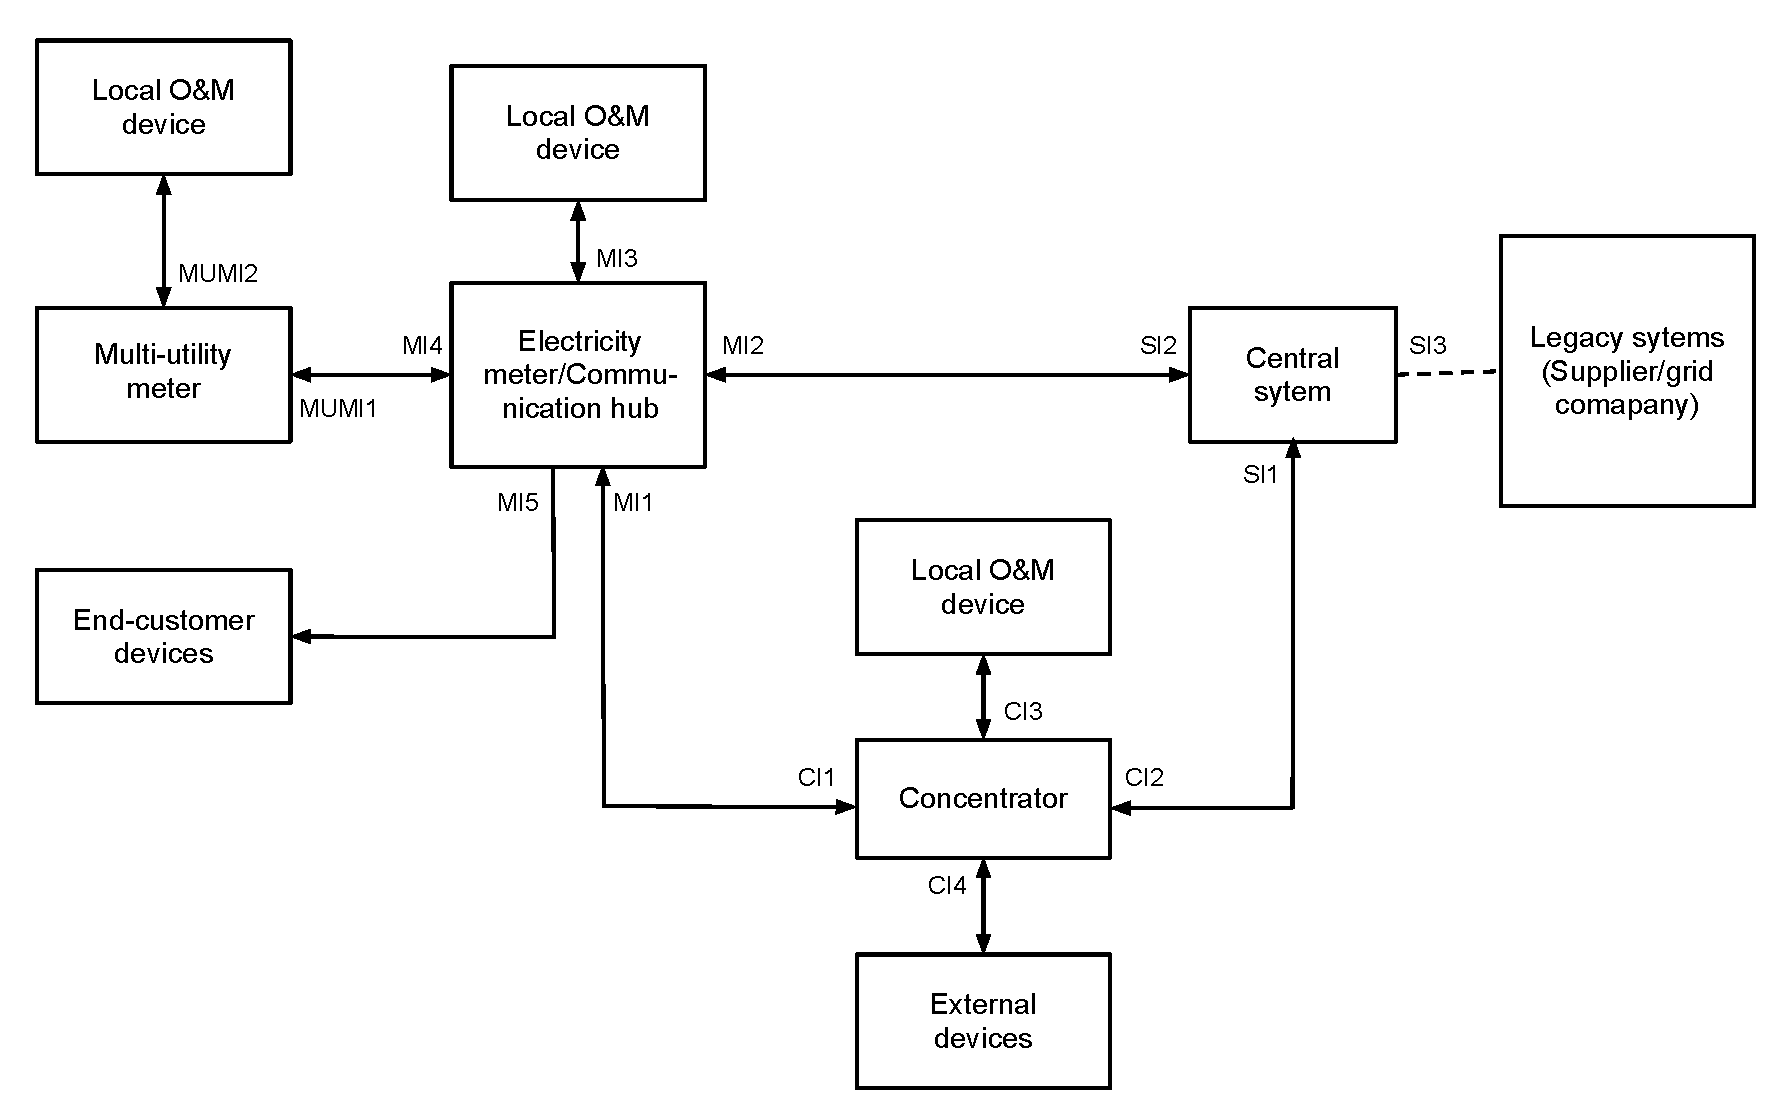
\includegraphics[width=0.8\textwidth]{images/OPEN_meter_arch}
\caption{OPEN meter system architecture \cite{OPEN_mtr_arch}.}
\label{fig:OPEN_sys_arch}
\end{figure}

\begin{table}[h!]
  \begin{center}
    \begin{tabular}{| p{3.5cm} | p{3cm} | p{4cm} |}
    \hline 
    Interface & Selected Technology Type & Lower Layer protocols \\
    \hline \hline
    MI1-CI1 & PLC & Prime, IEC 61334-5-1 \\
    \hline
    CI2-SI1 & Wireless & UMTS, GPRS \\
    \hline
    MI2-SI2 & Wireless & UMTS, GPRS \\
    \hline
    MI3, CI3 and MUMI2 & Wireless & IEE802.15.4,  IEE802.11-2007 \\
    \hline
    MUMI1-MI4 & Wireless & IEE802.15.4,  IEE802.11-2007, Wireless M-Bus \\
    \hline
    CI4 & Wireless & Zigbee, WiFi \\
    \hline
    MI5 & Wireless & Bluetooth, Zigbee \\
    \hline
    \end{tabular}
  \end{center}
  \caption{Technologies for the interfaces}
  \label{tab:OPEN_intf}
\end{table}

Electricity meter can act as a communication hub for other meters in the house and hence other meters could delegate certain power-intensive operations to the electricity meter such as cryptographic functions. The concentrator is need when the local n/w uses power line communications as a media. Local O\&M devices are used by the utilities personnel to locally configure, operate and maintain the meters and other electronic devices of the architecture. Table~\ref{tab:OPEN_intf} lists the various technologies chosen for the different interfaces in the system architecture.

Security is taken care by the DLMS/COSEM protocols. DLMS or Device Language Message Specification, is the suite of standards developed and maintained by the DLMS User Association and has been co-opted by the IEC TC13 WG14 into the IEC 62056 series of standards. COSEM or Companion Specification for Energy Metering, includes a set of specifications that defines the Transport and Application Layers of the DLMS protocol. 

%Chapter 5: Life Cycle Model
\chapter{Life cycle model}

A life cycle model is a representation of the major phases of a device during its lifetime and their interrelationships in a graphical framework that can be easily understood and communicated. 

The LFID and HFID are the two IDs embedded in a smart meter for the purpose of  distinguishing the frequency of transmission of the metered data. The LFID is used for transmitting the low frequency metered data and the utility can attribute the metered data to the individual customer and can be used for billing purposes. On the other hand the HFID is used to collect high frequency metered data however the data is anonymized.

The LFID and HFID values  are hard-coded into the smart meter, with only the manufacturer and/or the 3rd party escrow service being aware of their link within a single smart meter. They are held in the smart meter as part of the ID profiles.
PISM or Personally identifiable SM Profile containing:
PISM Certificate (CERT), containing LFID, PISM Public Key and PISM Certifying Authority infromation.
PISM Private Key


ANSM or Anonymous SM profile containing>
ANSM Certificate (CERT), containing HFID, ANSM Public Key and ANSM Certifying Authority information.
ANSM Private Key


A secure protocol using the PISM and ANSM are used to create a Client Data Profile (CDP) and Anonymous Data Profile(ADP). 


Participants in the SM-Network:
Smart Meter: Responsible for measuring the amount of electricity (commodity) consumed at defined intervals.

Gateway: Responsible for collecting metered data and the monitoring of proper functioning (weather the SM is dead or alive) of the connected SMs. Transmitting the thus collected data to the accounting company.

Accounting company: Responsible for collecting the data from all the Gateways under its jurisdiction and preparing billing information for each of the consumer.

Energy supplier / Utility: Responsible for power transmission to the consumers. This entity could also be a power generator, such as, a nuclear power plant or a thermal power plant. 

Different cases of installation of an SM:
A brand new SM to be installed at a consumer premises
A used SM to be installed at a consumer premises
A SM to be un-installed at a consumer premises


How is the communication between the SM and the gateway handled in the above three cases? More particularly the cryptographic key management between the SM and the Gateway.

Simple solution: Once the SM are assigned to a particular Accounting company then they are associated with that Accounting company for the rest of the life of the device.
Complex solution: An alternative would be to have a cheaper detachable hardware module within the SM such that once the SM changes hands from one accounting company to another, then the new accounting company replace the hardware module. This hardware module could be responsible for implementing the security scheme of a particular accounting company.

Before the installation / un-installation of the SM at a consumer premises it is assumed that the accounting company has received an application from the consumer,  at an earlier time period, requesting for a SM installation / un-installation. Thus a unique ID is stored in the SM before it is sent out to the field. This unique ID then helps the accounting company to establish an association between the consumer and a particular SM.

The frequency of data reporting from a particular SM is agreed upon during the initialization process b/w the SM and the Gateway. The Gateway then consolidates/aggregates the data and sends the low frequency (previously agreed upon) data to the accounting company and the high frequency data to the electricity company (via the accounting company). Here the Gateway serves  two purposes. Firstly, it helps is aggregating the fine grained metered data from each meter into coarse grained data. In other words the high frequency metered data is transformed into a low frequency reading which helps in creating the billing information. Secondly, the Gateway helps in concealing the association between a particular meter and its high frequency reading, to the accounting company.

Although the high frequency data is transferred via the accounting company to the electricity company, the confidentiality of the data is maintained using cryptography. By this way only the electricity company knows the association between a particular SM and its high frequency metering data. It is assumed that the information about association between an ID and the consumer is shared between the accounting company and the electricity company. This is required  in an event of discrepancy regarding the billing information.

Case 1: The smart meter is carried to the consumer premises by a installation technician. The technician connects the meter to the port mean for it. Once this is done, the meter receives a IP  address. Then it contacts the DNS with a special record request to find the IP of the nearest Gateway. The meter then establishes a connection with the Gateway using the IP address from the DNS query. The process of establishing the connection between the meter and the Gateway is detailed as follows:

<blah...blah...blah..>

The Gateway then communicates the necessary information, about the SM, to the accounting company, which then is responsible for associating the SM with a particular consumer.

Case 2: Similar to Case 1. However care has to be taken so that any previous data stored in the meter is not used for the new consumer so as to cause any discrepancies in the metering information.

Case 3: The technician authenticates himself to the meter as the un-installing procedure has to be carried out only by an authorized personnel. The authentication mechanism could be using  smart card, usb dongle or a password. The meter is taken out of the network by entering an un-install code known to the technician and the Gateway with which the meter was previously registered will delete and entry corresponding to the meter. Gateway then communicates this un-install information to the accounting system. The accounting system is then responsible for de-associating the meter with the consumer in its records. 

OPEN Meter project

Assumptions for the prototype:

Only electricity meter is considered and is assumed to be directly powered by the grid. However ideas/techniques to be listed on how to handle other utility meters which are most probably battery powered.

%References
\bibliographystyle{plain}
\bibliography{bibilography}

\end{document}
